%%%%%%%% ICML 2026 SUBMISSION %%%%%%%%%%%%%%%%%%%%
\documentclass{article}

\usepackage{microtype}
\usepackage{graphicx}
\usepackage{subcaption}
\usepackage{booktabs}
\usepackage{multirow}
\usepackage{xcolor}
\usepackage{hyperref}
\newcommand{\theHalgorithm}{\arabic{algorithm}}
\usepackage{icml2026}
\usepackage{amsmath}
\usepackage{amssymb}
\usepackage{mathtools}
\usepackage{amsthm}
\usepackage{algorithm}
\usepackage{algorithmic}
\usepackage[capitalize,noabbrev]{cleveref}

\graphicspath{{./figures/}{./figures_context/}{../outputs/context_generation/figures/}}

\newcommand{\X}{\mathcal{X}}
\newcommand{\D}{\mathcal{D}}
\newcommand{\M}{\mathcal{M}}
\newcommand{\E}{\mathbb{E}}
\newcommand{\1}{\mathbf{1}}

\icmltitlerunning{DMS-Conditioned Protein Diffusion}

\begin{document}

\twocolumn[
  \icmltitle{DMS-Conditioned Protein Diffusion for Multi-Mutant Design}

  \icmlsetsymbol{equal}{*}
  \begin{icmlauthorlist}
    \icmlauthor{Anonymous Authors}{anon}
  \end{icmlauthorlist}
  \icmlaffiliation{anon}{Anonymous Institution}
  \icmlcorrespondingauthor{Anonymous}{anon@anon.org}
  \icmlkeywords{protein design, diffusion language models, deep mutational scanning, controllable generation, experimental context}
  \vskip 0.3in
]

\printAffiliationsAndNotice{}

\begin{abstract}
Protein diffusion models can generate plausible sequences, but they are usually guided by generic reward models that do not know the experimental fitness landscape of the protein being engineered. In practice, many laboratories can measure a single-mutant deep mutational scanning map for a target protein, while exhaustive multi-mutant measurement remains combinatorially expensive. We introduce EditGuard-Diffusion, a DMS-conditioned protein diffusion framework that treats a target protein's single-mutant map as experimental context for multi-mutant generation. A frozen DPLM-650M backbone proposes masked edits, while a trained context adapter reads the mutation map and adds learned logit corrections at edit positions. The resulting system converts one-step experimental measurements into target-specific combinatorial design policies, and is evaluated against unguided DPLM, best-of-K reranking, additive DMS reranking, DMS-prior reranking, PhaseSMC, and measured-pool additive references on held-out ProteinGym and Megascale tasks.
\end{abstract}

\section{Introduction}

Modern protein generators are increasingly good at producing sequences that look natural under large protein language models \cite{wang2024dplm}. Protein engineering, however, is rarely a generic generation problem. A scientist usually cares about one protein, one assay, and one experimentally measured objective such as fluorescence, binding, activity, expression, or stability. Deep mutational scanning (DMS) provides exactly this kind of target-specific information by measuring thousands of single substitutions \cite{notin2024proteingym,tsuboyama2023mega}. The missing interface is generative. Current DMS workflows mostly predict variant effects, while current protein diffusion models mostly condition on sequence, structure, family, or learned reward models.

This paper studies the following problem. Given a wildtype sequence $x_0$ and a single-mutant DMS map $\M_g$ for protein $g$, generate multi-mutant variants $x$ that improve the measured objective while keeping edit risk controlled. This is the practical setting behind many combinatorial protein-engineering campaigns. Single substitutions reveal local experimental preferences, but useful variants often require multiple coordinated edits.

We introduce EditGuard-Diffusion, a DMS-conditioned adapter for protein diffusion language models. The adapter keeps DPLM-650M frozen and trains a small residual module that maps DPLM hidden states plus mutation-map context to amino-acid logit corrections. The design is intentionally simple. The goal is to test whether experimental mutation maps can function as prompts for protein diffusion models.

Our contributions are:
\begin{itemize}
  \item We formulate experimental-context protein generation, where a single-mutant DMS map conditions a generative protein model for multi-mutant design.
  \item We implement a frozen-DPLM context adapter trained on real multi-mutant measurements, with weighted masked-token likelihood and a pairwise ranking loss.
  \item We provide same-task baselines requested by reviewers, including unguided DPLM, best-of-K, additive DMS reranking, DMS-prior reranking, PhaseSMC, and measured-pool additive references.
  \item We preserve the earlier additive and calibration theory as an appendix-level justification for why single-mutant maps are informative, rather than as the main language of the paper.
\end{itemize}

\section{Problem Setup}

Let $x_0 \in \X$ be the wildtype sequence of length $L$. A single-mutant DMS map for protein $g$ is a partially observed matrix
\begin{equation}
  \M_g \in \mathbb{R}^{L \times 20},
\end{equation}
where $\M_g[p,a]$ records the measured effect of substituting amino acid $a$ at position $p$, when available. Let $O_g[p,a] \in \{0,1\}$ denote whether that measurement exists. The design task is to sample variants
\begin{equation}
  x \sim q_\theta(\cdot \mid x_0, \M_g, O_g, B),
\end{equation}
where $B$ is an edit budget. Evaluation uses held-out measured multi-mutants only. Single-mutant rows are available as context, while multi-mutant rows are never used in the target protein context.

\section{Method}

\subsection{Mutation-Map Context}

We convert the DMS map into a tensor with three parts. First, observed mutation scores are robust-normalized within the assay. Second, a binary observation mask records missing entries. Third, per-position summaries encode coverage, mean observed score, score spread, position index, and wildtype residue identity. The context vector at position $p$ is
\begin{equation}
  c_p =
  [\M_g[p,1:20], O_g[p,1:20], s_p] \in \mathbb{R}^{49}.
\end{equation}
The implementation rejects multi-mutant rows during context construction to prevent target-label leakage.

\subsection{Frozen-DPLM Adapter}

For a candidate edit mask $P=\{p_1,\ldots,p_B\}$, DPLM receives the wildtype sequence with those positions masked. Let $h_p$ be the frozen DPLM hidden state at masked position $p$, and let $\ell^{\mathrm{DPLM}}_p \in \mathbb{R}^{20}$ be the DPLM amino-acid logits restricted to standard residues. The adapter predicts a residual correction
\begin{equation}
  \Delta \ell_p =
  f_\theta(h_p, c_p, B),
\end{equation}
and samples from
\begin{equation}
  \ell^{\mathrm{ctx}}_p =
  \ell^{\mathrm{DPLM}}_p + \lambda \Delta \ell_p.
\end{equation}
The DPLM backbone is frozen. Only $f_\theta$ is trained.

\subsection{Training Objective}

Training uses measured multi-mutants from proteins in the training split. For a measured variant $x$ with substitutions at $P(x)$ and assay value $y(x)$, we mask all positions in $P(x)$ and maximize the likelihood of the observed alternate residues:
\begin{align}
  \mathcal{L}_{\mathrm{NLL}}(\theta)
  &=
  - \sum_{x \in \D_{\mathrm{train}}}
  w(y(x))
  \sum_{p \in P(x)}
  \log q_\theta\!\left(
    x_p \mid x_0, \M_g, P(x)
  \right).
\end{align}
We also use a within-batch pairwise ranking loss. For two variants $x_i,x_j$ from the same training batch with $y_i > y_j$, define the generated log-probability score $s_\theta(x)$ as the mean log-probability of its observed edited residues. The ranking term is
\begin{equation}
  \mathcal{L}_{\mathrm{rank}}(\theta)
  =
  \E_{y_i > y_j}
  \log(1 + \exp(-(s_\theta(x_i)-s_\theta(x_j)))).
\end{equation}
The full loss is
\begin{equation}
  \mathcal{L} = \mathcal{L}_{\mathrm{NLL}} + \eta \mathcal{L}_{\mathrm{rank}}.
\end{equation}

\begin{algorithm}[t]
\caption{DMS-Conditioned DPLM Generation}
\label{alg:context-generation}
\begin{algorithmic}
\STATE {\bfseries Input:} wildtype $x_0$, single-mutant map $\M_g$, edit budget $B$, frozen DPLM, adapter $f_\theta$
\STATE Build context vectors $c_p$ for every position
\FOR{mask pattern $P \subseteq \{1,\ldots,L\}$ with $|P|=B$}
  \STATE Mask positions $P$ in $x_0$
  \STATE Run frozen DPLM and extract $(h_p,\ell_p^{\mathrm{DPLM}})$ for $p \in P$
  \STATE Compute $\ell_p^{\mathrm{ctx}}=\ell_p^{\mathrm{DPLM}}+\lambda f_\theta(h_p,c_p,B)$
  \STATE Sample edited residues from $\ell_p^{\mathrm{ctx}}$ with hard residue constraints
\ENDFOR
\STATE Deduplicate variants and return ranked candidates
\end{algorithmic}
\end{algorithm}

\section{Experiments}

\textbf{Data.} We use ProteinGym DMS assays and Megascale single and double mutant measurements \cite{notin2024proteingym,tsuboyama2023mega}. The context for each target protein contains only single-mutant measurements. Evaluation uses measured multi-mutants held out from context construction.

\textbf{Baselines.} We compare against unguided DPLM, DPLM best-of-K, DPLM plus additive DMS reranking, DPLM plus the existing DMS function prior, PhaseSMC from the previous manuscript, and a measured-pool additive reference. The measured-pool reference is reported as an upper/reference baseline because it selects from measured variants rather than generating new sequences.

\textbf{Metrics.} We report labeled overlap, held-out hit rate, mean fitness, best fitness, mean edit distance, task constraint satisfaction, runtime, and stratified performance by edit budget.

\begin{figure}[t]
\centering
\fbox{\parbox{0.92\columnwidth}{\centering Figure 1 placeholder. Experimental mutation map as context for DPLM.}}
\caption{EditGuard-Diffusion treats a single-mutant DMS map as experimental context for protein diffusion.}
\label{fig:method}
\end{figure}

\begin{figure}[t]
\centering
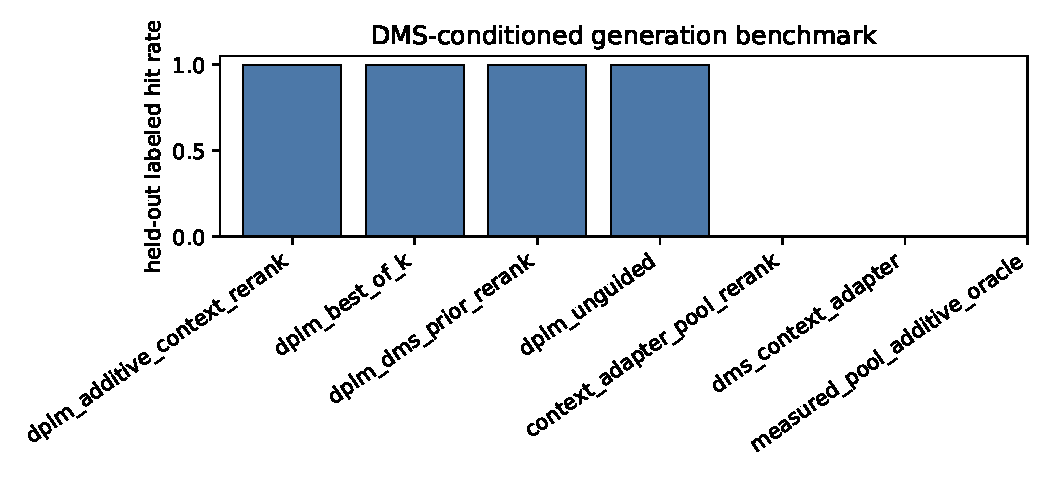
\includegraphics[width=\columnwidth]{fig3_context_generation_leaderboard.pdf}
\caption{Held-out benchmark leaderboard. This figure is generated from \texttt{outputs/context\_generation/context\_generation\_metrics.csv}.}
\label{fig:leaderboard}
\end{figure}

\section{Discussion}

The central question is whether laboratory mutation maps can be used like prompts for protein diffusion models. If the trained adapter improves over unguided DPLM and reranking baselines, the result establishes experimental-context generation as a practical interface between DMS and generative protein design. If additive DMS reranking remains strongest, the conclusion is still useful: single-mutant experimental maps are an unexpectedly hard baseline for protein diffusion, and future generative methods should be evaluated against them directly.

\section*{Impact Statement}

This work is intended to support protein-engineering hypothesis generation. Generated variants require experimental validation before use in clinical, therapeutic, or environmental settings.

\bibliographystyle{icml2026}
\bibliography{editguard_phase}

\newpage
\appendix
\onecolumn

\section{Implementation Status}

The current implementation adds:
\begin{itemize}
  \item \texttt{MutationMapContext}, a leakage-safe single-mutant DMS context tensor.
  \item \texttt{DMSContextAdapter}, a trainable residual logit adapter for frozen DPLM.
  \item Modal entrypoints for adapter training, generation, baseline evaluation, and figure construction.
\end{itemize}

\section{Relation to the Earlier PhaseSMC Manuscript}

The earlier manuscript studied additive composition and edit-distance calibration in detail. That material is useful as theory and as an ablation. It should not be the main language of the revised paper. The main paper should use field-standard terms: DMS, protein diffusion, experimental context, multi-mutant design, reranking, calibration, and held-out protein evaluation.

\end{document}
